\documentclass{jsarticle}
\usepackage[dvipdfmx]{graphicx}
\usepackage{float}
\usepackage{amsmath}
\usepackage[dvipdfmx]{color}
\usepackage{listings}
\usepackage{subfigure}
\begin{document}
\title{小野寺研インターン}
\author{澤 孝晃}
\maketitle

\section{序論}
\label{sec:intro}
トランジスタの微細化によりゲート長が7nmのデバイスが製造可能となっており、μm以下の寸法になってからは電子や分子の量子的な揺らぎが顕著になり、大量のトランジスタからなら集積回路のチップにおいて、同じ寸法のトランジスタ特性間にミスマッチが起きるようになった。ここで、素子同士の特性のミスマッチが回路の性能と信頼性にどう影響を与えるのかが重要である。製造時に発生する特性のミスマッチは静的ばらつきと認識されている一方、動作時にトランジスタの特性が時間によって変動することがありノイズや経年劣化として認識されている。ノイズの主要成分は熱雑音であり白色雑音とも呼ばれる。

主要成分の他に、結晶と結晶の界面に置いて、分子間結合の分子間結合の切断による欠陥が存在する。界面に存在する欠陥に自由キャリアの捕獲と放出が繰り返されると電流の時間変動が発生する。このような変動をフリッカーノイズと呼び、低い周波数領域に置いてパワー密度が大きいことが特徴である。MOSトランジスタの場合、シリコンと酸化膜の間の界面に存在する欠陥が原因となっている。トランジスタの寸法がμm以下になってから、各種欠陥へのキャリアのトラップによる影響が顕著に現れ始めた。その理由として、欠陥1つへのキャリアのトラップの相対的な影響が顕著にあらわれたことと、製造技術の進歩により各種欠陥の数が減少してきており、あるトランジスタに欠陥が存在する確率が減少してきたことがある。従って、1つの欠陥がチャネルに流れる電流にどう影響されるか正確に見積もる手法が求められるようになった。相対的に大きな電流変動は、1つの欠陥への1つの欠陥へのキャリアの捕獲と放出の減少により発生するため離散的な変動として観測される。また、その変動が起きる時間間隔は固定ではなく大きくばらつく。

ランダムテレグラフノイズ(RTN)は界面に存在するトラップにキャリアの捕獲・放出によりデバイスの閾値電圧が変動する現象である。閾値電圧だけでなく移動度が変化する説もある。RTNを特徴付けるパラメータは、トラップあたりのオン電流の変化量、トラップあたりの時定数、トラップの数の3種類がある。トラップあたりのRTNパラメータを評価するのではなく、RTNによる合計量の変動を評価し、その変動量の分布をモデル化することにより回路設計に活かすことを目標にする。



\section{方法}
\label{sec:method}

今回のインターンでは、微細デバイスに発生するRTNをリング発振回路を用いて測定し、RTNが回路性能の最悪分布に与える影響を評価する。測定対象であるRTNは統計的な性質を持っており、各種統計的な性質をモデル化することが目的である。統計的な評価を行うために、同じ寸法の大量のデバイスの電流特性の時間変化を測定し、デバイス毎に観測される電流値変動の振幅および捕獲・放出するまでの平均時間などを評価する。

今回の測定環境では、FPGAボードとPCを使って、スロット0からスロット71のリングオシレータ(RO)を、セクション0からセクション383まで384個のセクションの発信周波数を測定する。各セクション10秒ずつ測定するので、合計1時間程度かかる。また、ROの電源は0.5Vに設定する。また、以下の表\ref{table:circuit}に示されているROについて測定を行なった。ゲート幅や負荷容量が異なっていて、段数は特に指定されていない限り7段である。

\begin{table}[hbtp]
  \caption{各回路の構造}
  \label{table:circuit}
  \centering
  \begin{tabular}{c|l|c|c}
    \hline
    Index  & Cell Name & Slot number & Description \\
    \hline
    \multicolumn{4}{c}{Section Left} \\
    \hline
    1 & FM\_RIGHT\_RING7\_P140\_N140\_MAHFUZ & 0-1, 28-35 & Balanced, no extra load \\ 
    2 & FM\_LEFT\_RING7\_P655X16\_N140\_MAHFUZ & 2 & N skewed \\
    3 & FM\_LEFT\_RING7\_P655X16\_N280\_MAHFUZ & 4 & N skewed \\
    4 & FM\_LEFT\_RING7\_P655X16\_N560\_MAHFUZ & 6 & N skewed \\
    5 & FM\_LEFT\_RING7\_P655X16\_N1120\_MAHFUZ & 8 & N skewed \\
    6 & FM\_LEFT\_RING7\_P655X16\_N2240\_MAHFUZ & 10 & N skewed \\
    7 & FM\_LEFT\_RING7\_P140\_N420X16\_MAHFUZ & 12 & P skewed \\
    8 & FM\_LEFT\_RING7\_P280\_N420X16\_MAHFUZ & 14 & P skewed \\
    9 & FM\_LEFT\_RING7\_P560\_N420X16\_MAHFUZ & 16 & P skewed \\
    10 & FM\_LEFT\_RING7\_P1120\_N420X16\_MAHFUZ & 18 & P skewed \\
    11 & FM\_LEFT\_RING7\_P2240\_N420X16\_MAHFUZ & 20 & P skewed \\
    12 & FM\_LEFT\_RING7\_LE5O\_MK61INVXL1\_NAKAI & 25 & Medium size \\
    13 & FM\_LEFT\_RING7\_LE5O\_MK61INVXT11\_NAKAI & 26 & Large size \\
    \hline
    \multicolumn{4}{c}{Section Right} \\
    \hline
    14 & FM\_RIGHT\_RING7\_P140\_N140\_MAHFUZ & 36, 41-44, 49-71 & Balanced, no extra load \\
    15 & FM\_RIGHT\_RING7\_P280\_N280\_MAHFUZ & 37 & Balanced, no extra load \\
    16 & FM\_RIGHT\_RING7\_P560\_N560\_MAHFUZ & 38 & Balanced, no extra load \\
    17 & FM\_RIGHT\_RING7\_P1120\_N1120\_MAHFUZ & 39 & Balanced, no extra load \\
    18 & FM\_RIGHT\_RING7\_P2240\_N2240\_MAHFUZ & 40 & Balanced, no extra load \\
    19 & FM\_RIGHT\_RING7\_P140\_N140\_LOADXC1\_MAHFUZ & 46 & Extra load (small) \\
    20 & FM\_RIGHT\_RING7\_P140\_N140\_LOADXE1\_MAHFUZ & 47 & Extra load (medium) \\
    21 & FM\_RIGHT\_RING7\_P140\_N140\_LOADXL1\_MAHFUZ & 48 & Extra load (large) \\
    \hline
  \end{tabular}
\end{table}

\section{結果}
\label{sec:result}

以下の5種類の項目について結果を取得した。
\begin{itemize}
	\item
	nFETのゲート幅を変化させた場合
	\item
	pFETのゲート幅を変化させた場合
	\item
	nFETとpFETのゲート幅を変化させた場合
	\item
	段数を変化させた場合
	\item
	負荷容量を変化させた場合
\end{itemize}

\subsection{nFETのゲート幅を変化させた場合}
\label{sec:result_nFET}

発信周波数のヒストグラムを図\ref{fig:histogram_in_p_655}に示す。横軸は分周期にかけられた発振周波数で縦軸はその周波数を示した回数を表している。

\begin{figure}[hbtp]
	\centering
	\subfigure[n=140]{
		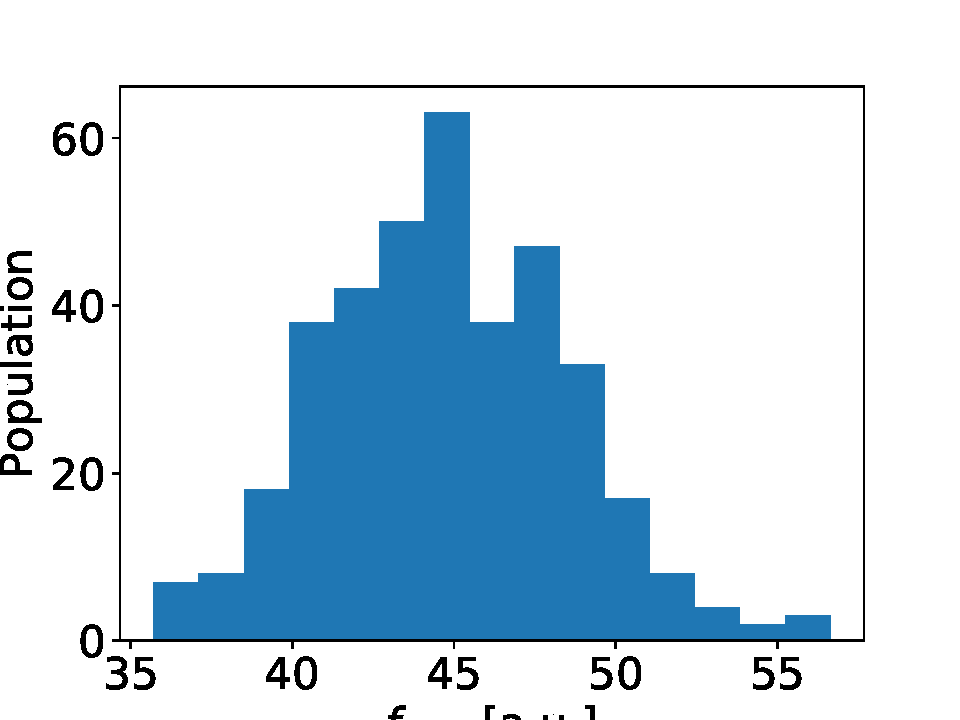
\includegraphics[width=5cm]{../../images/fig_max_hist/p655/180518_ch02v050r2d3_int44_time10000_fig_max_hist.pdf}
		\label{fig:hist_n_140}
	}
	\subfigure[n=280]{
		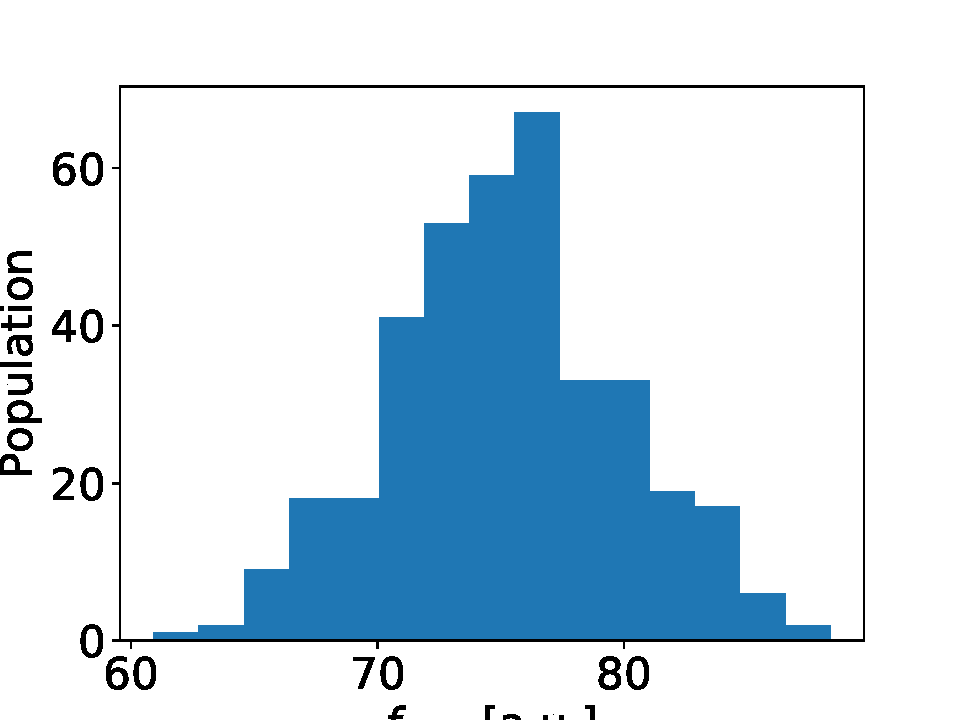
\includegraphics[width=5cm]{../../images/fig_max_hist/p655/180518_ch02v050r4d3_int74_time10000_fig_max_hist.pdf}
		\label{fig:hist_n_280}
	}
	\subfigure[n=560]{
		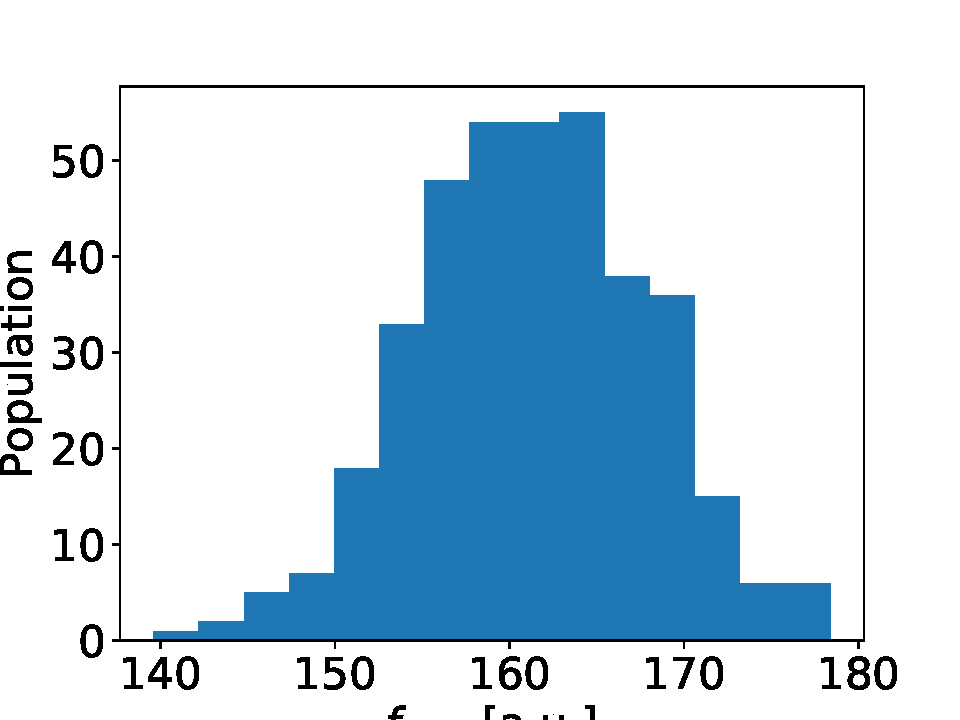
\includegraphics[width=5cm]{../../images/fig_max_hist/p655/180518_ch02v050r6d3_int160_time10000_fig_max_hist.pdf}
		\label{fig:hist_n_560}
	}
	\subfigure[n=1120]{
		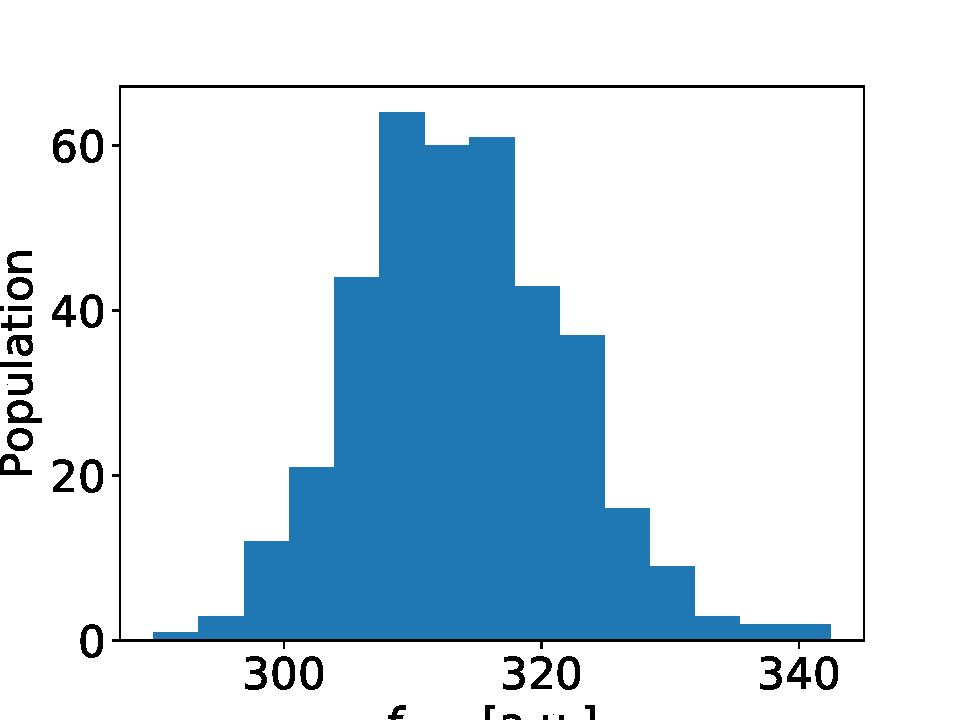
\includegraphics[width=5cm]{../../images/fig_max_hist/p655/180518_ch02v050r8d3_int313_time10000_fig_max_hist.pdf}
		\label{fig:hist_n_1120}
	}
	\subfigure[n=2240]{
		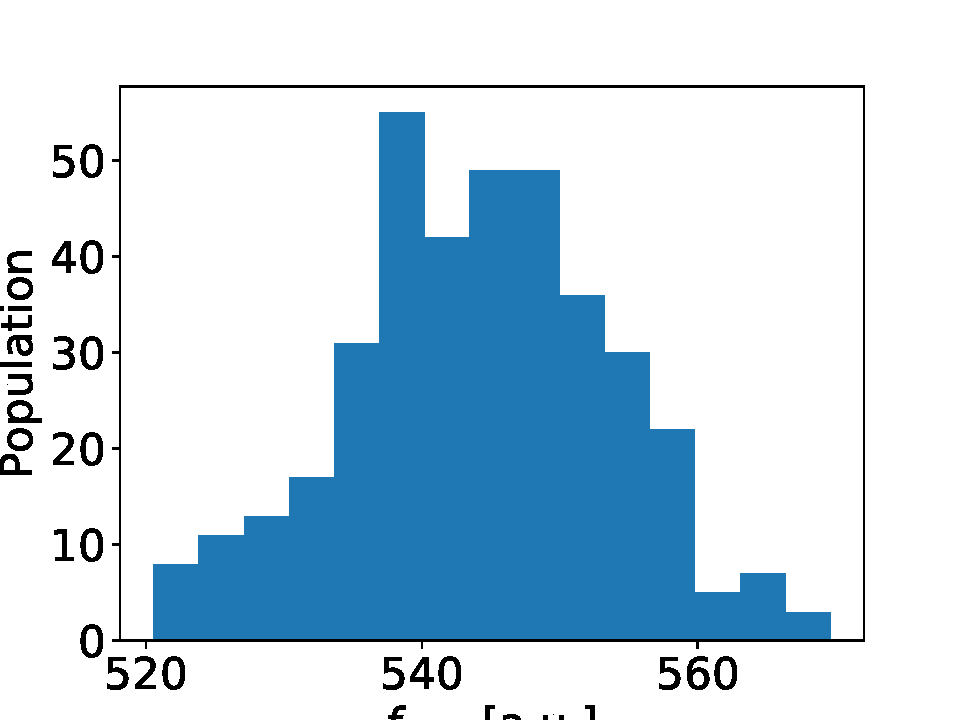
\includegraphics[width=5cm]{../../images/fig_max_hist/p655/180518_ch02v050r10d3_int543_time10000_fig_max_hist.pdf}
		\label{fig:hist_n_2240}
	}
	\caption{histogram in p = 655}
	\label{fig:histogram_in_p_655}
\end{figure}

分周した発振周波数のqqplotを図\ref{fig:qqplot_in_p_655}に示す。qqplotとは得られたデータと理論分布を比較し、その類似度を調べるためのグラフである。横軸は各分周器にかけられた発振周波数の各セクションでの最大値と最小値の差を最大値で割った値である。縦軸は理論分位数となっている。また、対数正規分布における$\sigma$と$\mu$を図\ref{fig:slope_intercept_in_p_655}に示す。また、a, bの値は横軸の値の対数を取った時の近似曲線の傾きと切片である。

\begin{figure}[hbtp]
	\centering
	\includegraphics[width=15cm]{../../images/anotation/p655.pdf}
	\caption{qqplot in p = 655}
	\label{fig:qqplot_in_p_655}
\end{figure}

\begin{figure}[hbtp]
	\centering
	\includegraphics[width=13cm]{../../least_squares/p655.png}
	\caption{slope intercept in p = 655}
	\label{fig:slope_intercept_in_p_655}
\end{figure}

図\ref{fig:qqplot_in_p_655}と図\ref{fig:slope_intercept_in_p_655}を見ると、nFETのゲート幅が大きくなればなるほど$\mu$の値は小さくなり、$\sigma$の値が大きくなっていることがわかる。 また, $\Delta F / F_{max}$の値が大きい所と小さいところで対数正規分布に従わなくなっている。ここで、n=140の時の$\Delta F / F_{max}$が大きい2点(s = 314, 192)と小さい2点(s = 233, 276)でのセクションにおける波形とタイムラグプロットを図\ref{fig:waveform_in_p_655_n_280}, \ref{fig:timelag_in_p_655_n_280}に示す。

\begin{figure}[hbtp]
	\centering
	\includegraphics[width=15cm]{../../images/waveform/p655_n280.pdf}
	\caption{waveform in p = 655 and n = 280}
	\label{fig:waveform_in_p_655_n_280}
\end{figure}

\begin{figure}[hbtp]
	\centering
	\includegraphics[width=15cm]{../../images/timelag/p655_n280.pdf}
	\caption{timelag plot in p = 655 and n = 280}
	\label{fig:timelag_in_p_655_n_280}
\end{figure}

図\ref{fig:waveform_in_p_655_n_280}におけるs=314, 192の時の結果を見ると何点かが離散的な値になっており、図\ref{fig:timelag_in_p_655_n_280}におけるs=314, 192の時の結果を見ると相関がない値が何点かある。これはRTNによる影響であると考えられる。$\Delta F / F_{max}$が小さい点(s = 233, 276)において対数正規分布に従っていないが、図\ref{fig:waveform_in_p_655_n_280}, \ref{fig:timelag_in_p_655_n_280}を考慮すると、白色雑音による影響がありRTNの影響のみを取り出すことができていないと考えられる。

同様にして、n=2240の時の時の$\Delta F / F_{max}$が大きい2点(s = 92, 295)と小さい2点(s = 205, 257)でのセクションにおける波形とタイムラグプロットを図\ref{fig:waveform_in_p_655_n_2240}, \ref{fig:timelag_in_p_655_n_2240}に示す。この図においても$\Delta F / F_{max}$が大きい2点(s = 92, 295)で離散的なを取っていてn=280の時と同じ現象が観測される。

\begin{figure}[hbtp]
	\centering
	\includegraphics[width=15cm]{../../images/waveform/p655_n2240.pdf}
	\caption{waveform in p = 655 and n = 2240}
	\label{fig:waveform_in_p_655_n_2240}
\end{figure}

\begin{figure}[hbtp]
	\centering
	\includegraphics[width=15cm]{../../images/timelag/p655_n2240.pdf}
	\caption{timelag plot in p = 655 and n = 2240}
	\label{fig:timelag_in_p_655_n_2240}
\end{figure}

\subsection{pFETのゲート幅を変化させた場合}
\label{sec:result_pFET}

発信周波数のヒストグラムを図\ref{fig:histogram_in_n_420}に示す。横軸は分周期にかけられた発振周波数で縦軸はその周波数を示した回数を表している。

\begin{figure}[hbtp]
	\centering
	\subfigure[p=140]{
		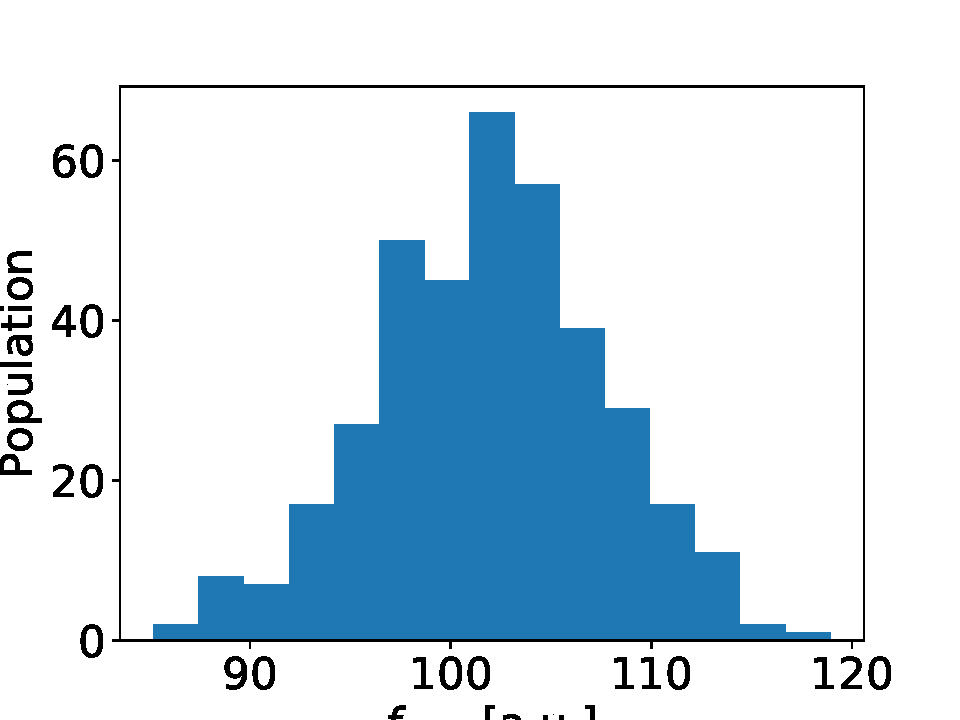
\includegraphics[width=5cm]{../../images/fig_max_hist/n420/180518_ch02v050r12d3_int101_time10000_fig_max_hist.pdf}
		\label{fig:hist_p_140}
	}
	\subfigure[p=280]{
		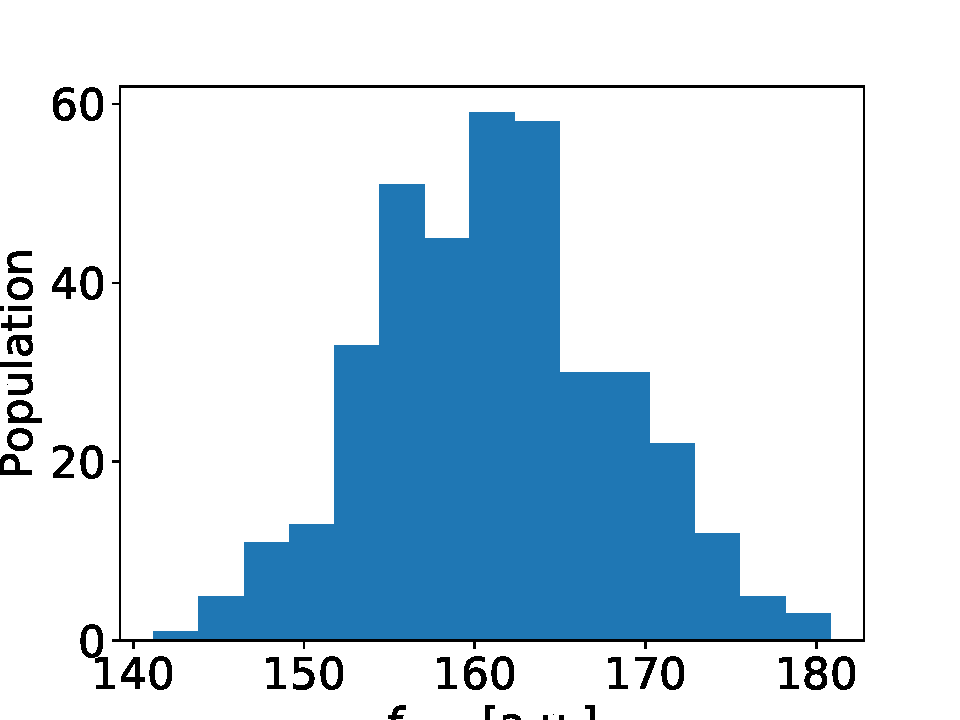
\includegraphics[width=5cm]{../../images/fig_max_hist/n420/180518_ch02v050r14d3_int160_time10000_fig_max_hist.pdf}
		\label{fig:hist_p_280}
	}
	\subfigure[p=560]{
		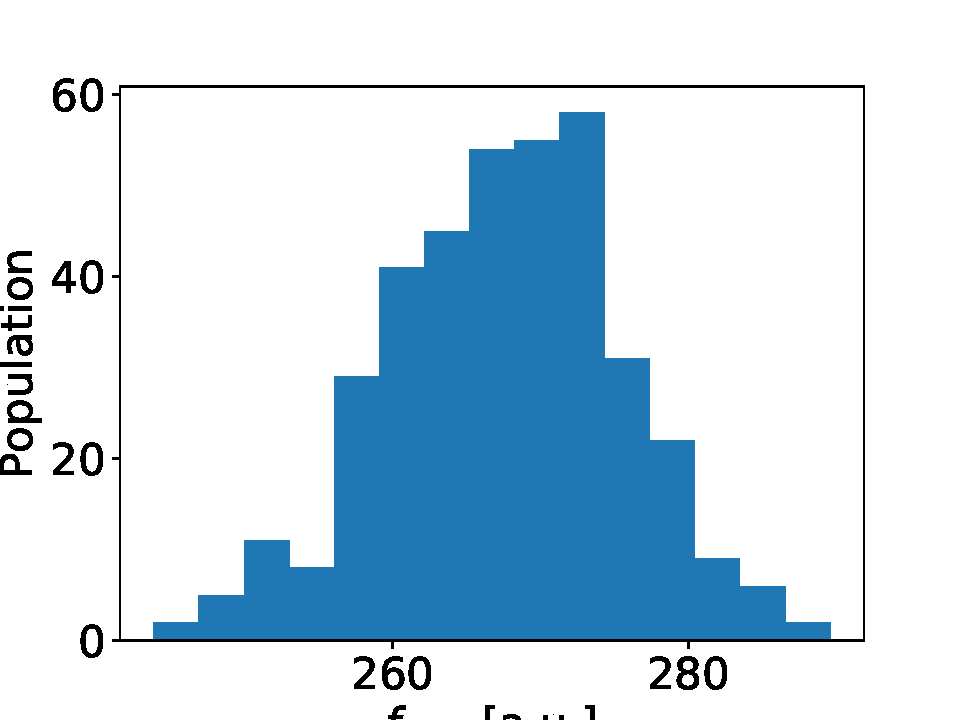
\includegraphics[width=5cm]{../../images/fig_max_hist/n420/180518_ch02v050r16d3_int266_time10000_fig_max_hist.pdf}
		\label{fig:hist_p_560}
	}
	\subfigure[p=1120]{
		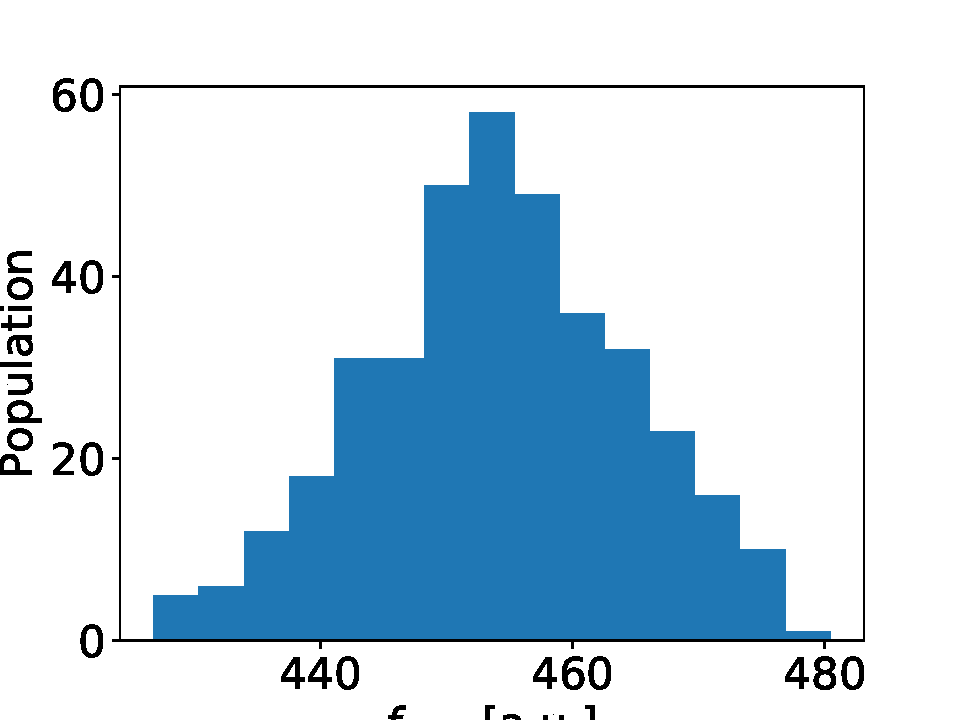
\includegraphics[width=5cm]{../../images/fig_max_hist/n420/180518_ch02v050r18d3_int453_time10000_fig_max_hist.pdf}
		\label{fig:hist_p_1120}
	}
	\subfigure[p=2240]{
		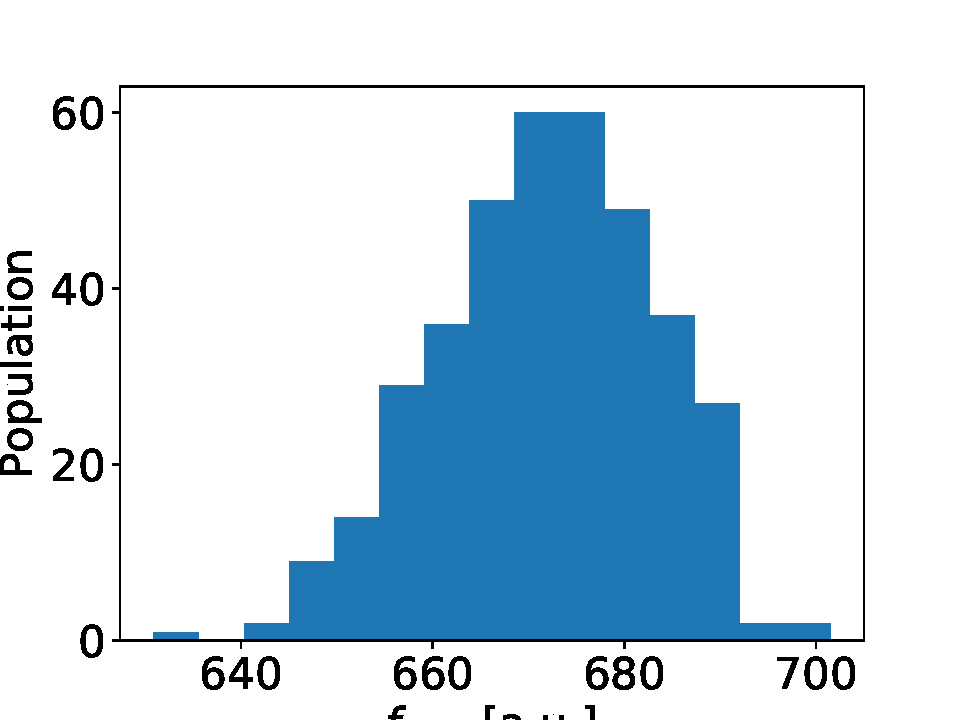
\includegraphics[width=5cm]{../../images/fig_max_hist/n420/180519_ch02v050r20d3_int671_time10000_fig_max_hist.pdf}
		\label{fig:hist_p_2240}
	}
	\caption{histogram in n = 420}
	\label{fig:histogram_in_n_420}
\end{figure}

分周した発振周波数のqqplotを図\ref{fig:qqplot_in_n_420}に、対数正規分布における$\sigma$と$\mu$を図\ref{fig:slope_intercept_in_n_420}に示す。\ref{sec:result_nFET}と比較するとほぼ同じ結果が見られる。

\begin{figure}[hbtp]
	\centering
	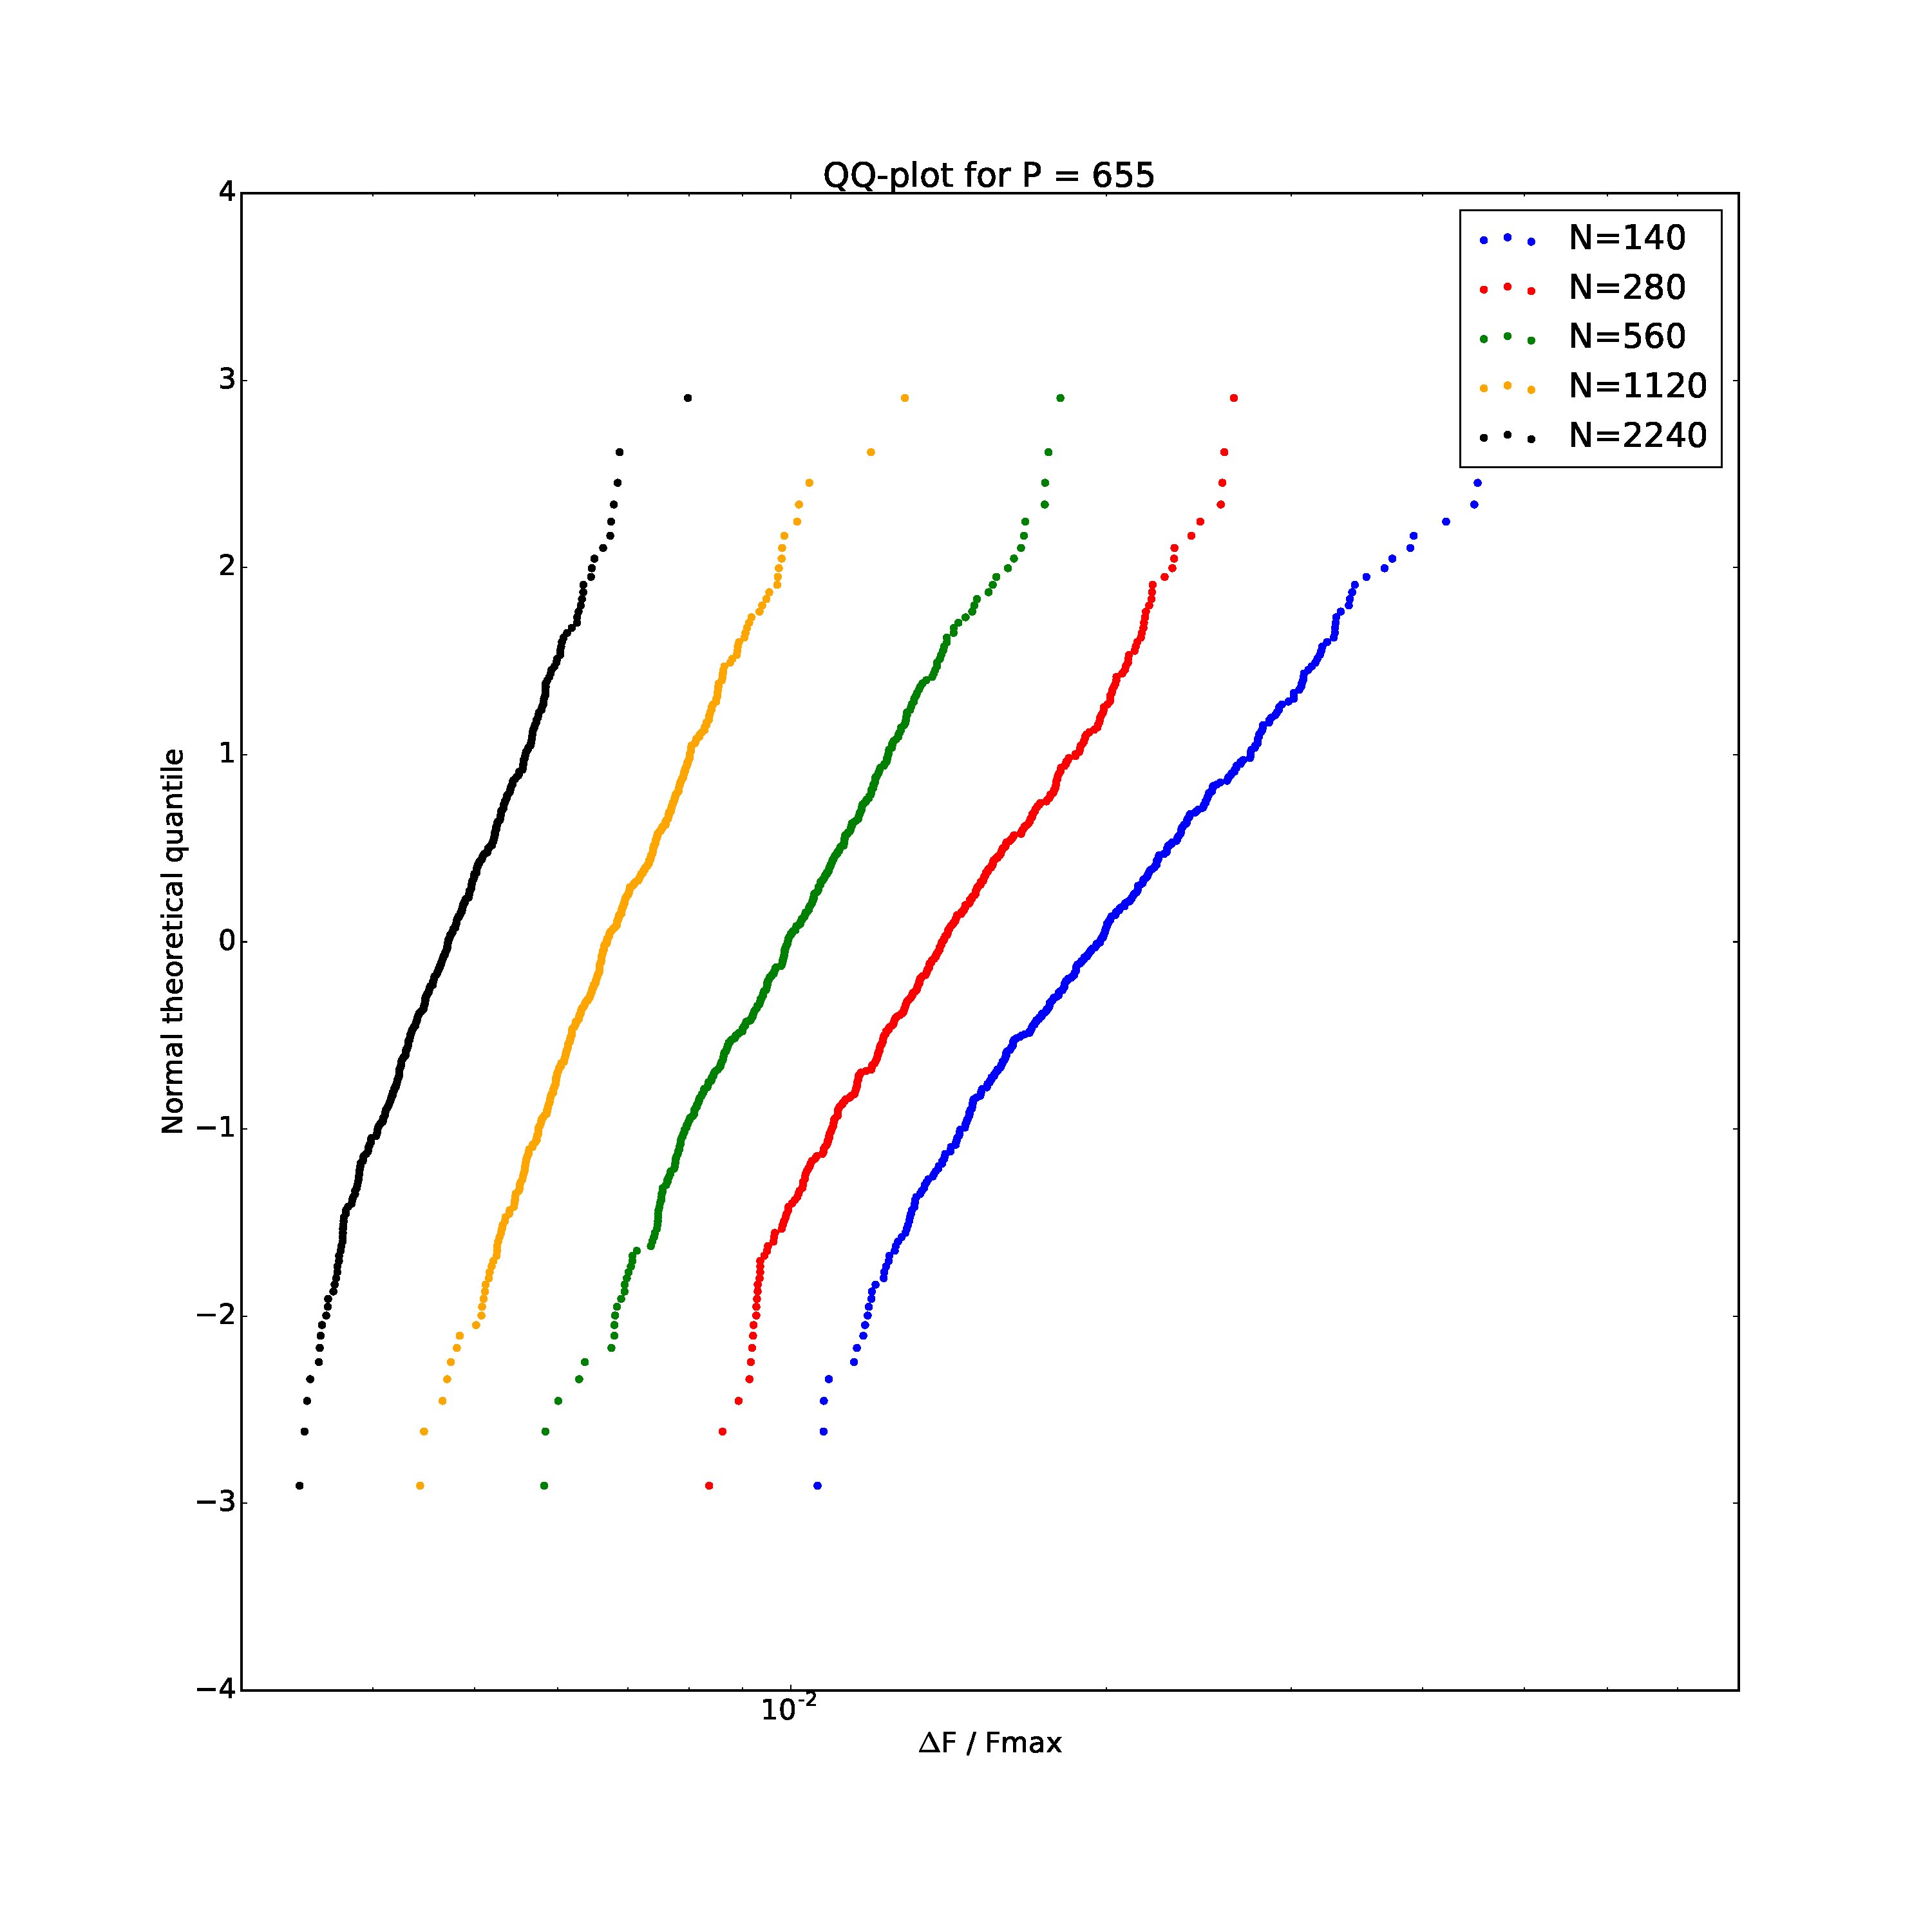
\includegraphics[width=15cm]{../../images/anotation/n420.pdf}
	\caption{qqplot in n = 420}
	\label{fig:qqplot_in_n_420}
\end{figure}

\begin{figure}[hbtp]
	\centering
	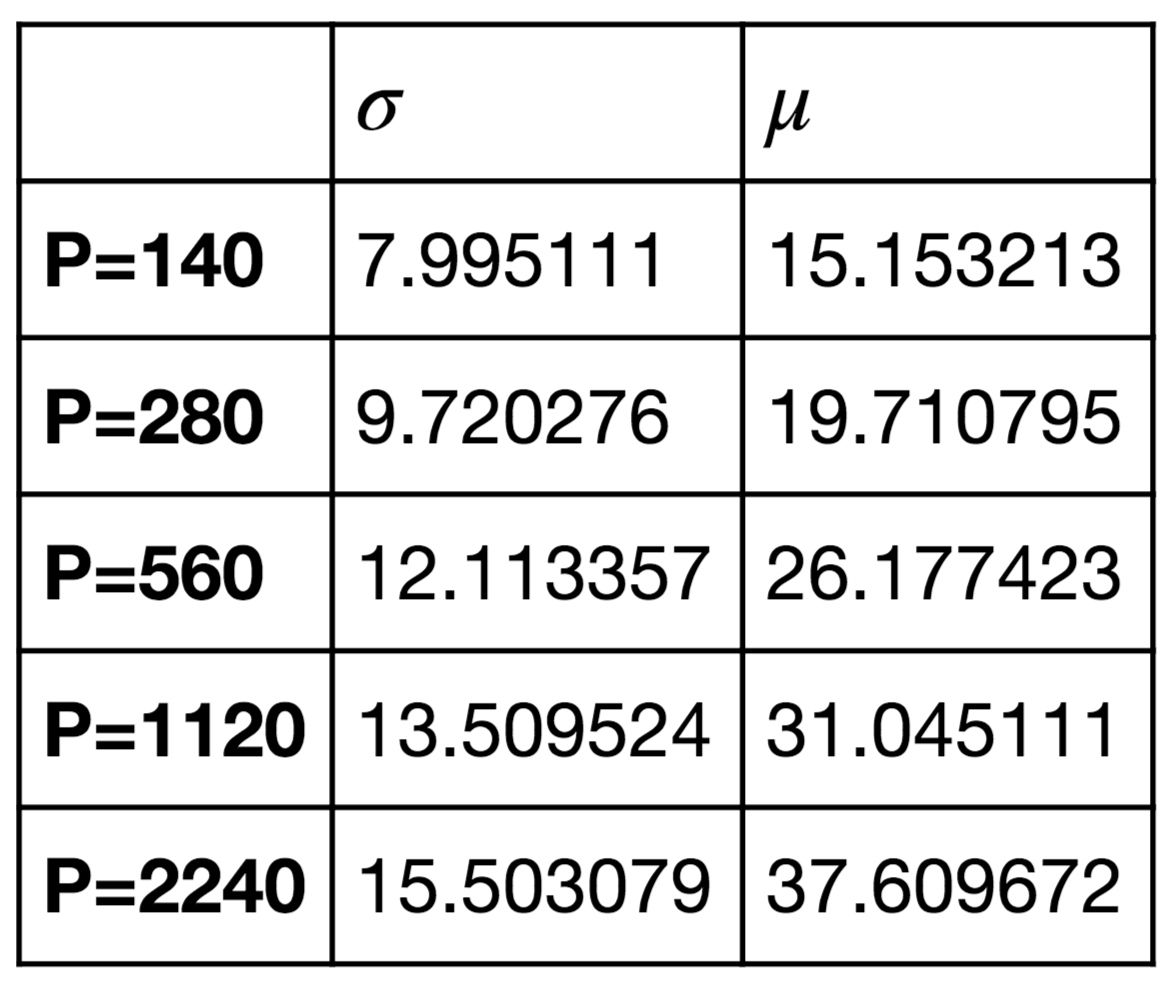
\includegraphics[width=13cm]{../../least_squares/n420.png}
	\caption{slope intercept in n = 420}
	\label{fig:slope_intercept_in_n_420}
\end{figure}


\subsection{nFETとpFETのゲート幅を変化させた場合}
\label{sec:result_nFET_pFET}

発信周波数のヒストグラムを図\ref{fig:histogram_in_square}に示す。横軸は分周期にかけられた発振周波数で縦軸はその周波数を示した回数を表している。

\begin{figure}[hbtp]
	\centering
	\subfigure[n, p=140]{
		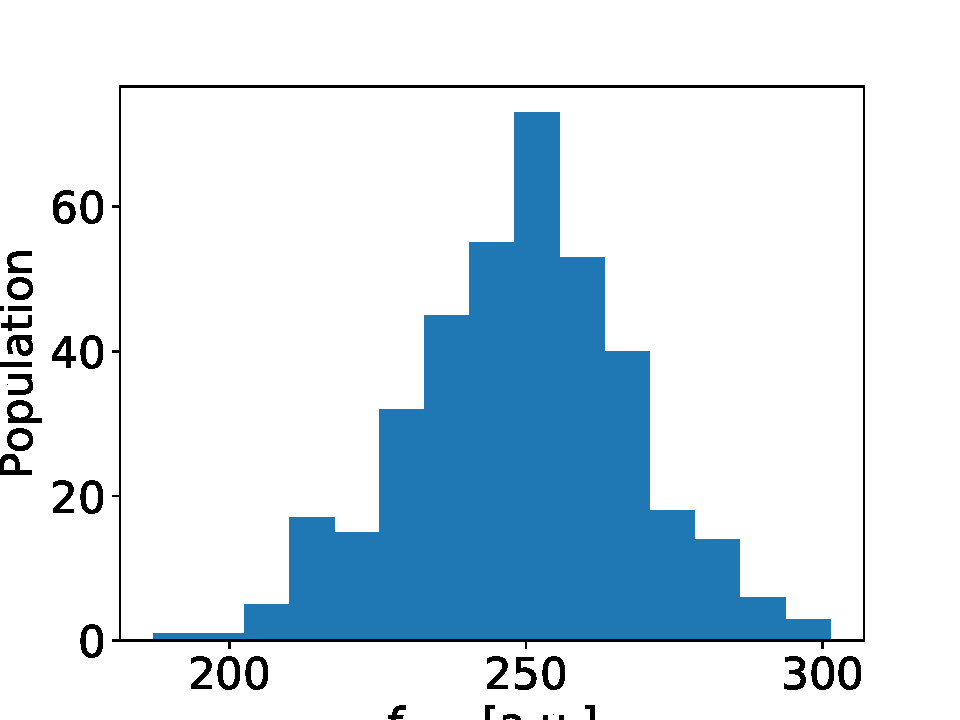
\includegraphics[width=5cm]{../../images/fig_max_hist/square/180522_ch02v050r36d3_int247_time10000_fig_max_hist.pdf}
		\label{fig:hist_n_p_140}
	}
	\subfigure[n, p=280]{
		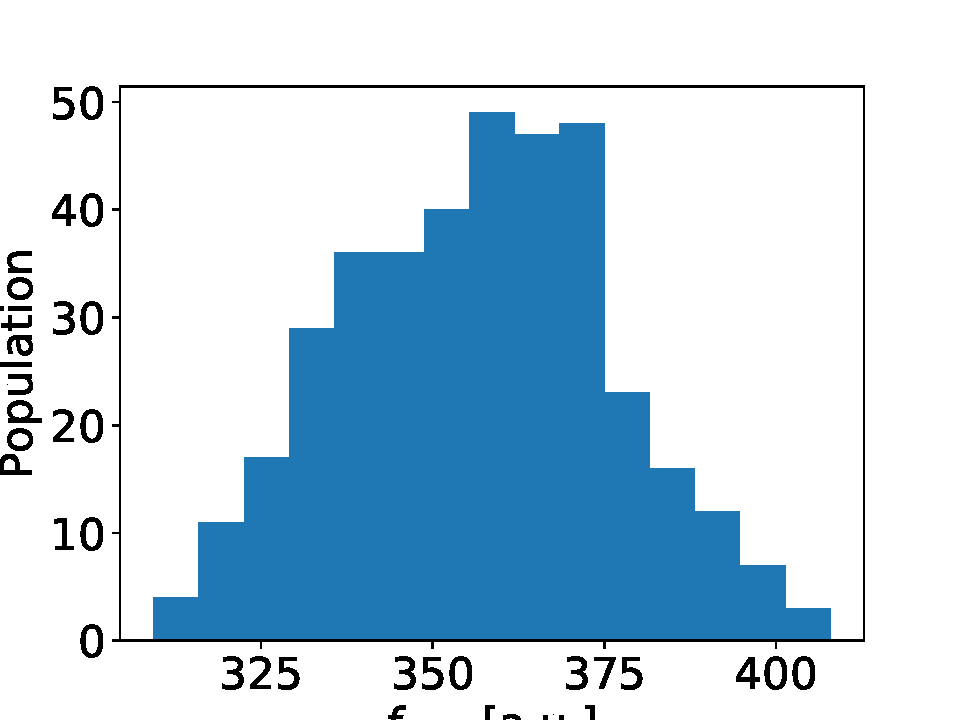
\includegraphics[width=5cm]{../../images/fig_max_hist/square/180522_ch02v050r37d3_int354_time10000_fig_max_hist.pdf}
		\label{fig:hist_n_p_280}
	}
	\subfigure[n, p=560]{
		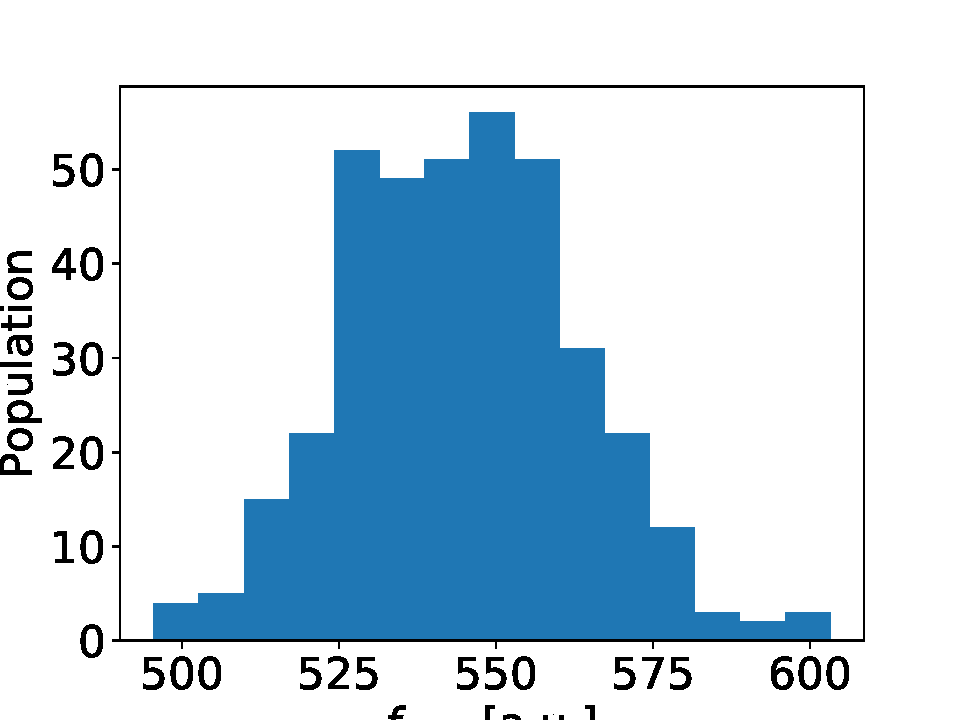
\includegraphics[width=5cm]{../../images/fig_max_hist/square/180522_ch02v050r38d3_int543_time10000_fig_max_hist.pdf}
		\label{fig:hist_n_p_560}
	}
	\subfigure[n, p=1120]{
		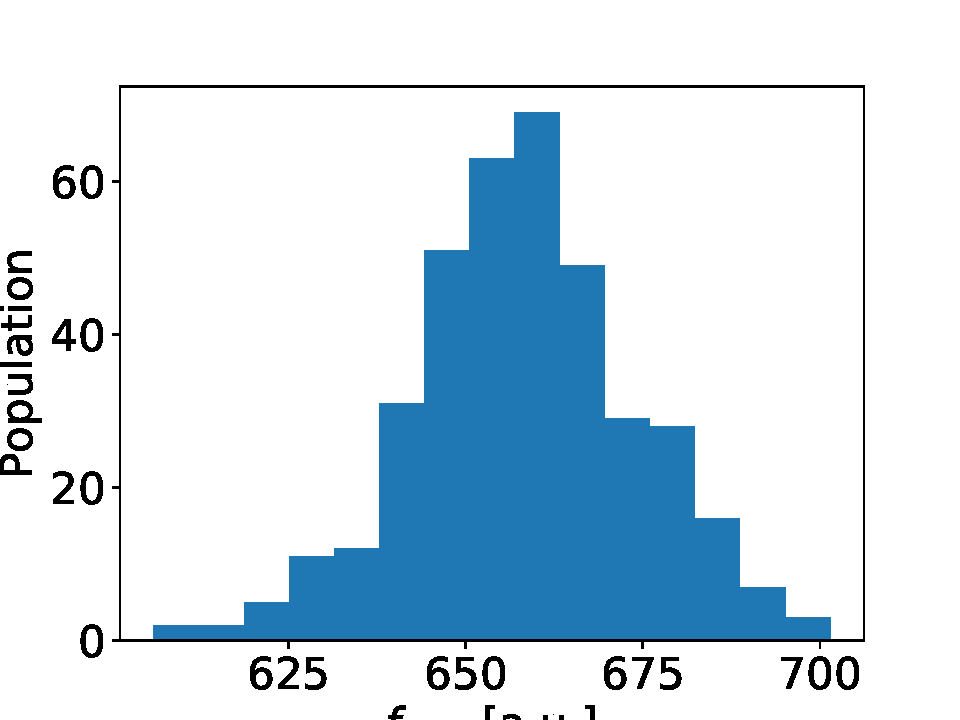
\includegraphics[width=5cm]{../../images/fig_max_hist/square/180522_ch02v050r39d3_int657_time10000_fig_max_hist.pdf}
		\label{fig:hist_n_p_1120}
	}
	\subfigure[n, p=2240]{
		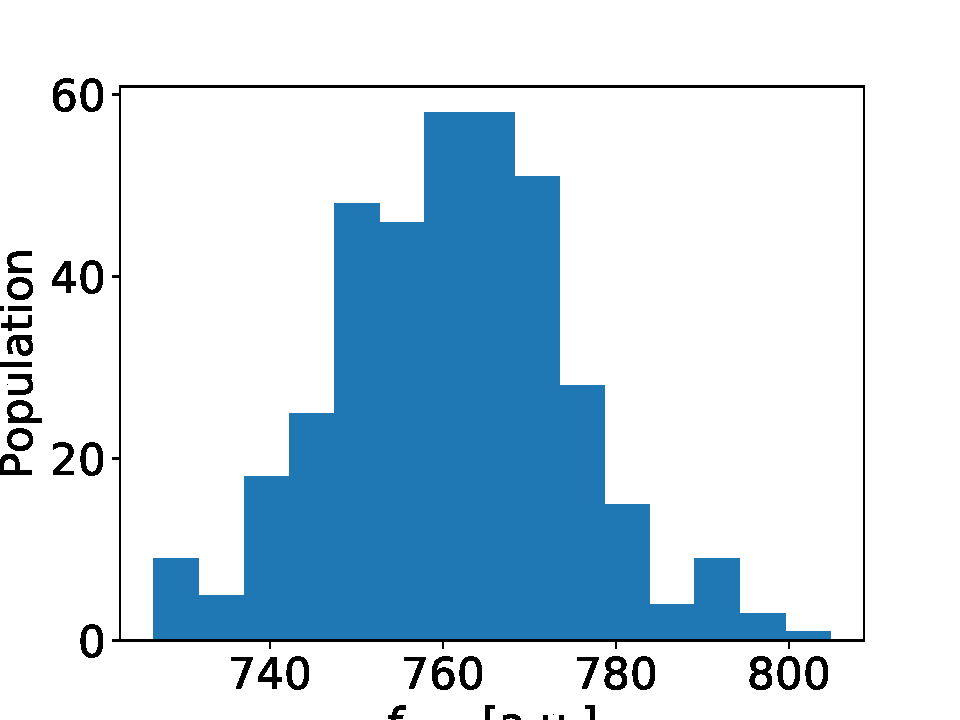
\includegraphics[width=5cm]{../../images/fig_max_hist/square/180522_ch02v050r40d3_int760_time10000_fig_max_hist.pdf}
		\label{fig:hist_n_p_2240}
	}
	\caption{histogram in square}
	\label{fig:histogram_in_square}
\end{figure}

分周した発振周波数のqqplotを図\ref{fig:qqplot_in_square}に、対数正規分布における$\sigma$と$\mu$を図\ref{fig:slope_intercept_in_square}に示す。\ref{sec:result_nFET}\ref{sec:result_pFET}と比較すると、n, p = 140, 280での結果について$\Delta F / F_{max}$の値が小さいところで対数正規分布からだいぶ離れてしまっている。これはゲート幅が小さいため白色雑音の影響を受けやすいからだと考えられる。

\begin{figure}[hbtp]
	\centering
	\includegraphics[width=15cm]{../../images/anotation/square.pdf}
	\caption{qqplot in square}
	\label{fig:qqplot_in_square}
\end{figure}

\begin{figure}[hbtp]
	\centering
	\includegraphics[width=13cm]{../../least_squares/square.png}
	\caption{slope intercept in square}
	\label{fig:slope_intercept_in_square}
\end{figure}


\subsection{段数を変化させた場合}
\label{sec:result_stage}

発信周波数のヒストグラムを図\ref{fig:histogram_in_load}に示す。横軸は分周期にかけられた発振周波数で縦軸はその周波数を示した回数を表している。

\begin{figure}[hbtp]
	\centering
	\subfigure[stage = 7]{
		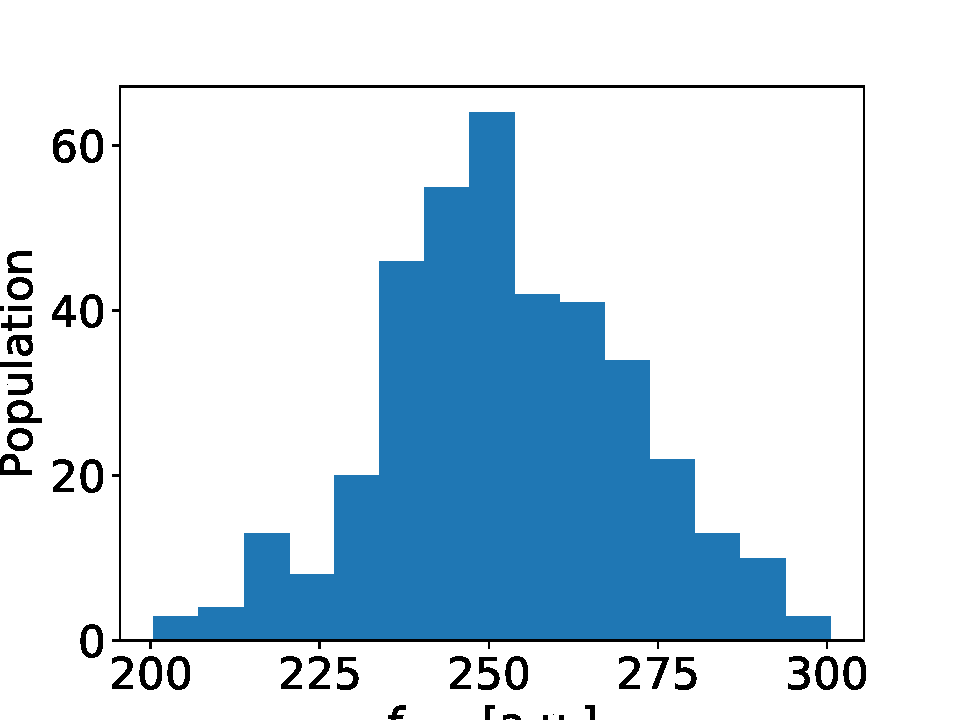
\includegraphics[width=5cm]{../../images/fig_max_hist/stage/180522_ch02v050r35d3_int250_time10000_fig_max_hist.pdf}
		\label{fig:hist_stage_7}
	}
	\subfigure[stage = 13]{
		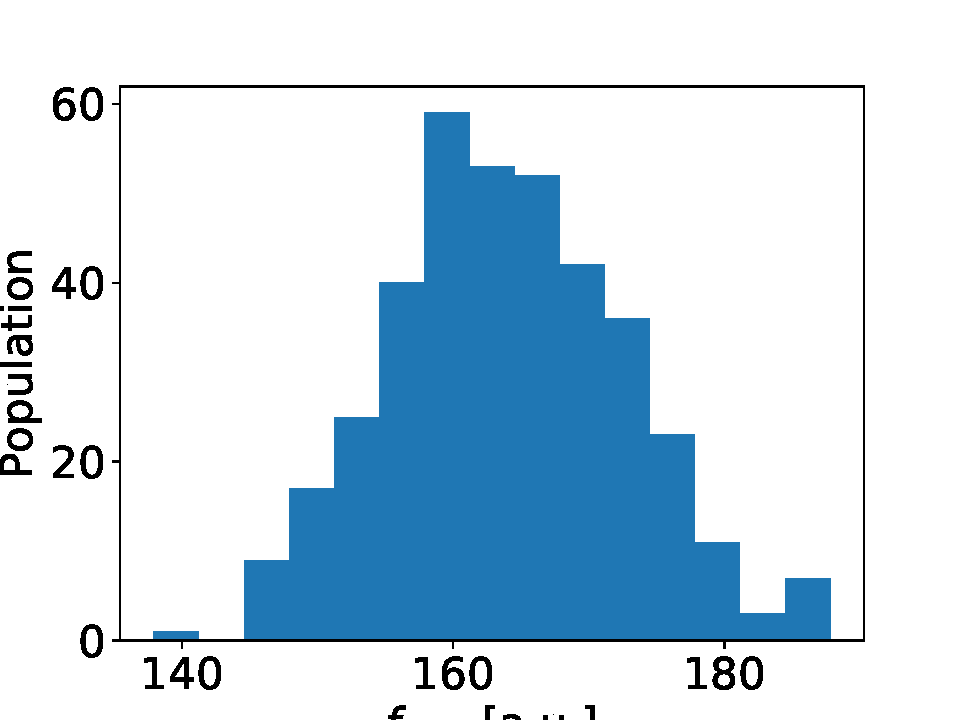
\includegraphics[width=5cm]{../../images/fig_max_hist/stage/180522_ch02v050r41d3_int163_time10000_fig_max_hist.pdf}
		\label{fig:hist_stage_13}
	}
	\subfigure[stage = 19]{
		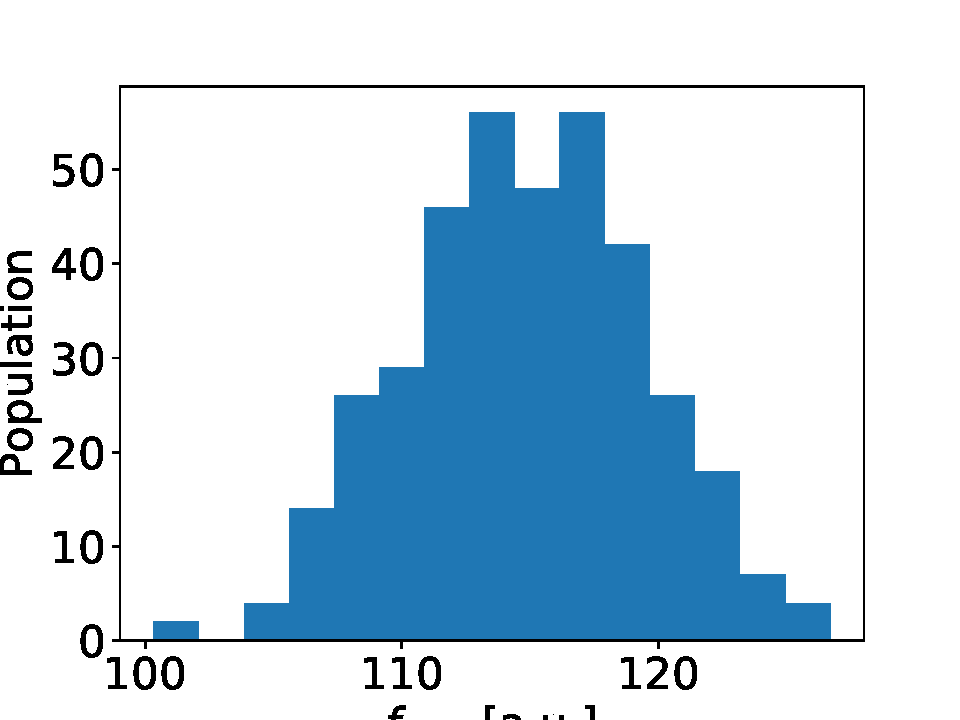
\includegraphics[width=5cm]{../../images/fig_max_hist/stage/180522_ch02v050r42d3_int114_time10000_fig_max_hist.pdf}
		\label{fig:hist_stage_19}
	}
	\subfigure[stage = 29]{
		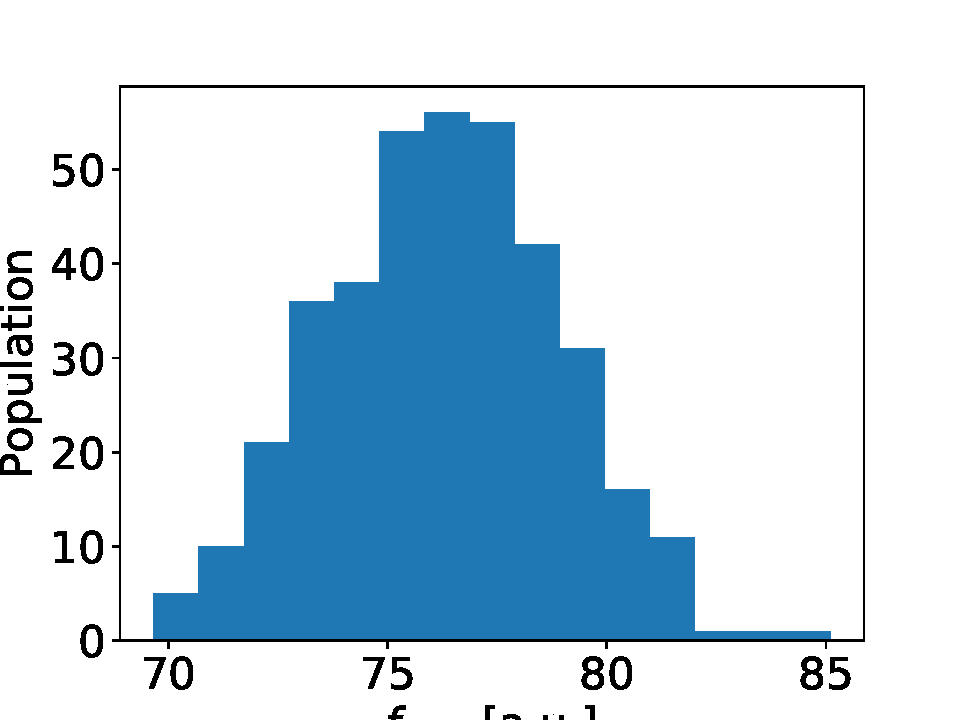
\includegraphics[width=5cm]{../../images/fig_max_hist/stage/180522_ch02v050r43d3_int75_time10000_fig_max_hist.pdf}
		\label{fig:hist_stage_29}
	}
	\subfigure[stage = 59]{
		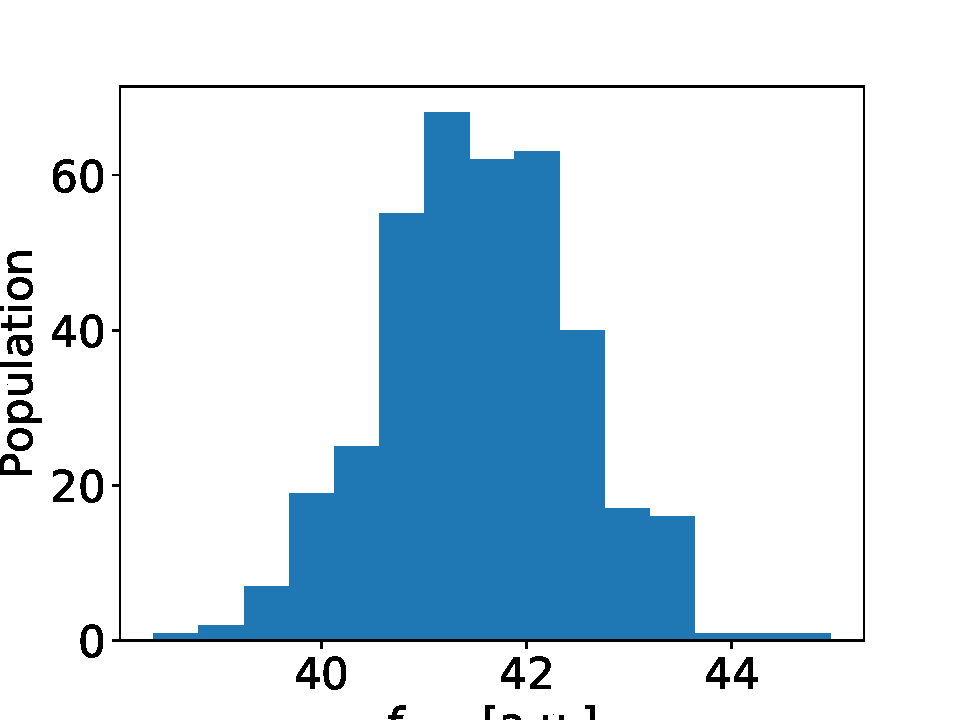
\includegraphics[width=5cm]{../../images/fig_max_hist/stage/180522_ch02v050r44d3_int41_time10000_fig_max_hist.pdf}
		\label{fig:hist_stage_59}
	}
	\caption{histogram in stage}
	\label{fig:histogram_in_stage}
\end{figure}

分周した発振周波数のqqplotを図\ref{fig:qqplot_in_stage}に、対数正規分布における$\sigma$と$\mu$を図\ref{fig:slope_intercept_in_stage}に示す。図からわかるように段数が大きくなればなるほど対数正規分布に近づいていることがわかる。

\begin{figure}[hbtp]
	\centering
	\includegraphics[width=15cm]{../../images/anotation/stage.pdf}
	\caption{qqplot in stage}
	\label{fig:qqplot_in_stage}
\end{figure}

\begin{figure}[hbtp]
	\centering
	\includegraphics[width=13cm]{../../least_squares/stage.png}
	\caption{slope intercept in stage}
	\label{fig:slope_intercept_in_stage}
\end{figure}

\subsection{負荷容量を変化させた場合}
\label{sec:result_stage}

発信周波数のヒストグラムを図\ref{fig:histogram_in_stage}に示す。横軸は分周期にかけられた発振周波数で縦軸はその周波数を示した回数を表している。

\begin{figure}[hbtp]
	\centering
	\subfigure[load = none]{
		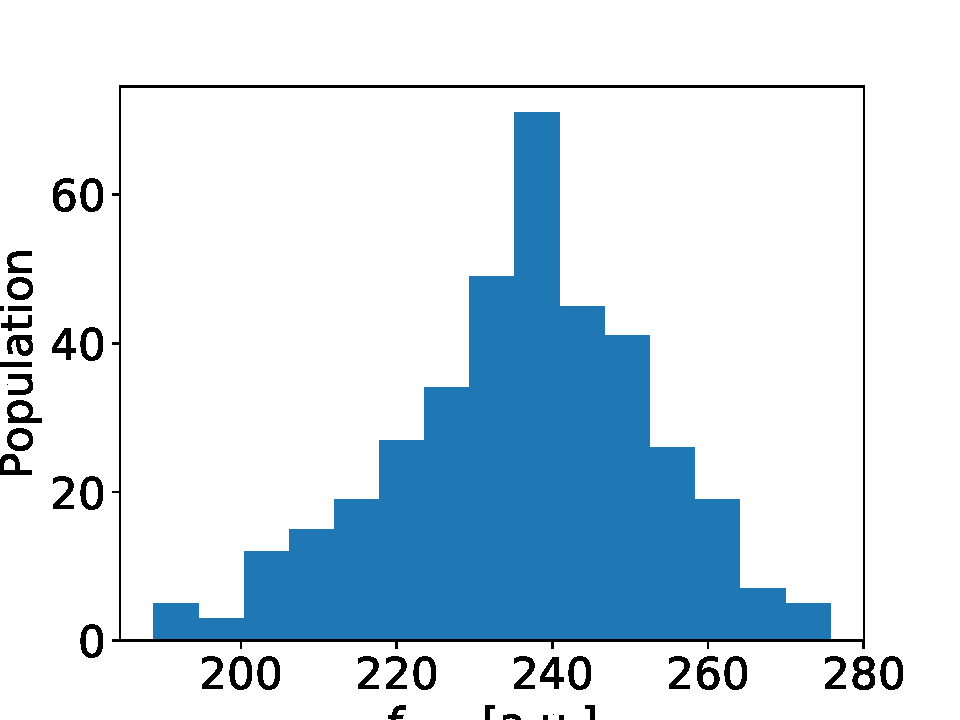
\includegraphics[width=5cm]{../../images/fig_max_hist/load/180522_ch02v050r49d3_int234_time10000_fig_max_hist.pdf}
		\label{fig:hist_load_29}
	}
	\subfigure[load = small]{
		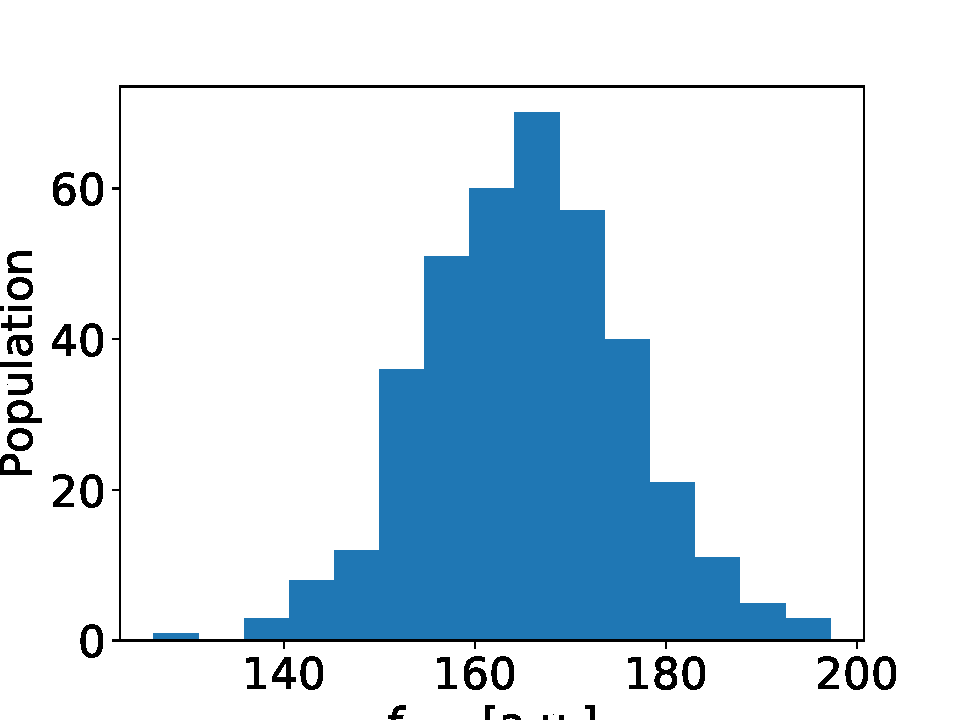
\includegraphics[width=5cm]{../../images/fig_max_hist/load/180522_ch02v050r46d3_int164_time10000_fig_max_hist.pdf}
		\label{fig:hist_load_7}
	}
	\subfigure[load = medium]{
		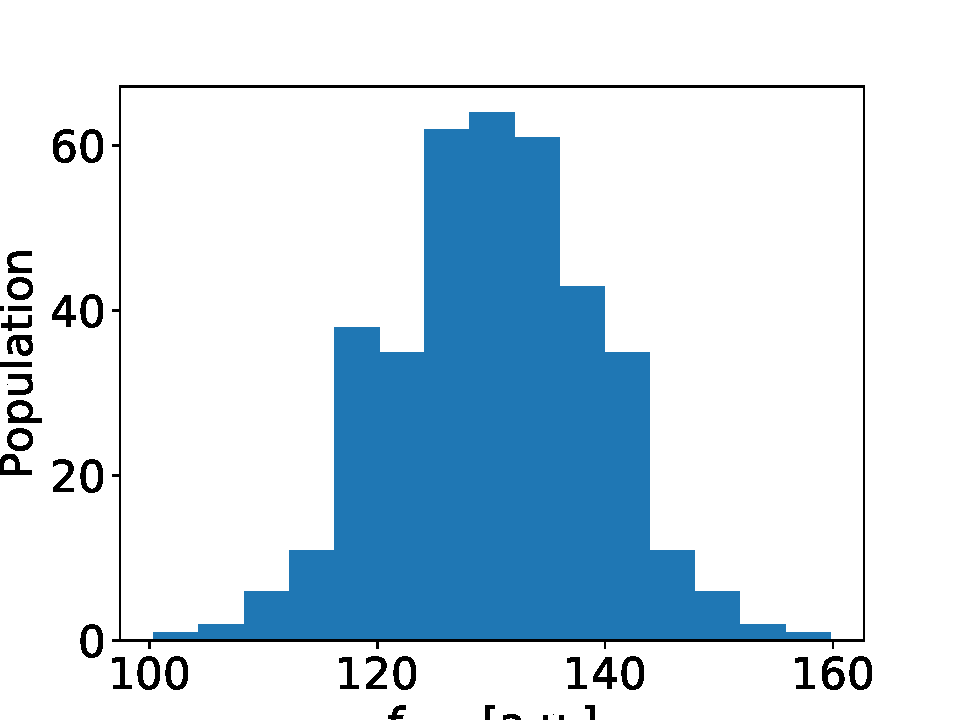
\includegraphics[width=5cm]{../../images/fig_max_hist/load/180522_ch02v050r47d3_int129_time10000_fig_max_hist.pdf}
		\label{fig:hist_load_13}
	}
	\subfigure[load = large]{
		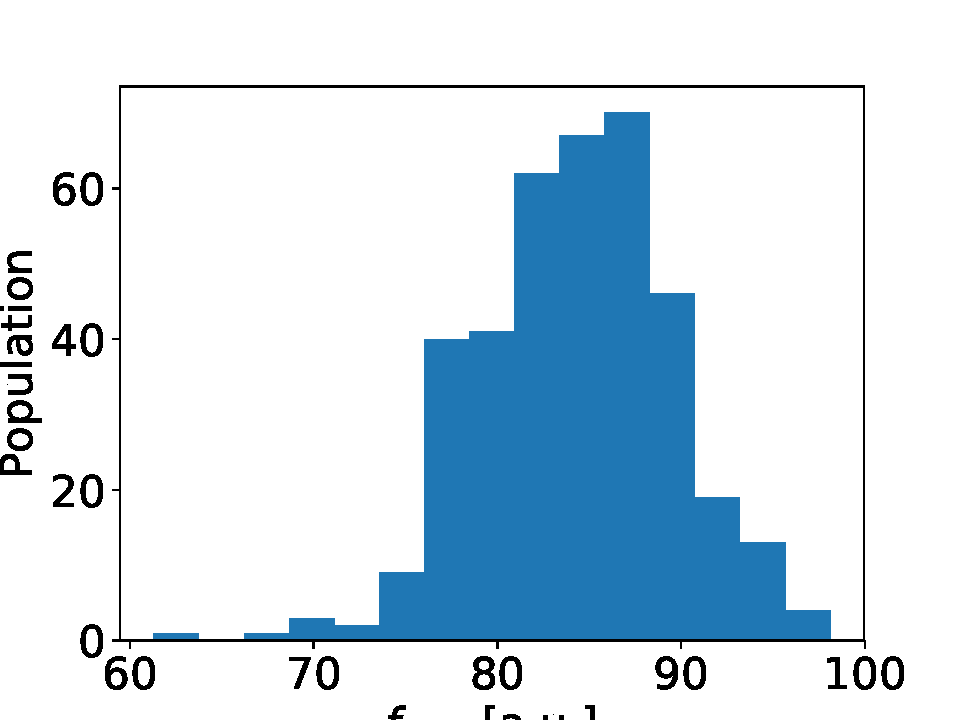
\includegraphics[width=5cm]{../../images/fig_max_hist/load/180522_ch02v050r48d3_int83_time10000_fig_max_hist.pdf}
		\label{fig:hist_load_19}
	}
	\caption{histogram in load}
	\label{fig:histogram_in_load}
\end{figure}

分周した発振周波数のqqplotを図\ref{fig:qqplot_in_load}に、対数正規分布における$\sigma$と$\mu$を図\ref{fig:slope_intercept_in_load}に示す。負荷容量がある場合を比べたときに負荷容量の大きさにかかわらずほとんど同じ特性を示した。

\begin{figure}[hbtp]
	\centering
	\includegraphics[width=15cm]{../../images/anotation/load.pdf}
	\caption{qqplot in load}
	\label{fig:qqplot_in_load}
\end{figure}

\begin{figure}[hbtp]
	\centering
	\includegraphics[width=13cm]{../../least_squares/load.png}
	\caption{slope intercept in load}
	\label{fig:slope_intercept_in_load}
\end{figure}

load=largeの時の$\Delta F / F_{max}$が大きい2点(s = 193, 285)と小さい2点(s = 282, 136)でのセクションにおける波形とタイムラグプロットを図\ref{fig:waveform_in_load_large}, \ref{fig:timelag_in_load_large}に、load=noneの時の$\Delta F / F_{max}$が大きい2点(s = 323, 283)と小さい2点(s = 0, 36)でのセクションにおける波形とタイムラグプロットを図\ref{fig:waveform_in_load_large}, \ref{fig:timelag_in_load_large}に示す。どちらも$\Delta F / F_{max}$が大きい2点にてRTNが発生していることが観測される。また負荷容量がない場合は負荷容量が大きい場合に比べて、RTNの発生頻度が高く、離散変動幅が大きいことがわかる。

\begin{figure}[hbtp]
	\centering
	\includegraphics[width=15cm]{../../images/waveform/load_large.pdf}
	\caption{waveform in large load}
	\label{fig:waveform_in_load_large}
\end{figure}

\begin{figure}[hbtp]
	\centering
	\includegraphics[width=15cm]{../../images/timelag/load_large.pdf}
	\caption{timelag plot in large load}
	\label{fig:timelag_in_load_large}
\end{figure}

\begin{figure}[hbtp]
	\centering
	\includegraphics[width=15cm]{../../images/waveform/load_none.pdf}
	\caption{waveform in none load}
	\label{fig:waveform_in_load_none}
\end{figure}

\begin{figure}[hbtp]
	\centering
	\includegraphics[width=15cm]{../../images/timelag/load_none.pdf}
	\caption{timelag plot in none load}
	\label{fig:timelag_in_load_none}
\end{figure}

\section{作成したスクリプト}

今回作成したスクリプトはipynbファイルであるのでjupyter notebookを使って実行する。基本的にはqqplot\_wid\_rtn.pyとplot\_rtn\_waveform.pyを改良して作成した。

\begin{itemize}
	\item
	qqplot\_wid\_rtn\_xscale.ipynb
	\begin{itemize}
		\item
		matファイルを4-5種類選択して実行すれば、qqplotとそれに対する最小二乗法を用いた近似直線、$\sigma$や$\mu$などの値が得られる。
		\item
		各点にはセクション番号のアノテーションが振られているので波形を見るときに参照できる
	\end{itemize}
	\item
	plot\_rtn\_waveform.ipynb
	\begin{itemize}
		\item
		matファイルを1種類選択し、セクション番号を4つ指定すればその波形とタイムラグプロットを見ることができる
	\end{itemize}


\end{itemize}

\section{まとめ}

今回のインターンでRTNの観測データを分析するスクリプトを書いてさまざまな評価を行いました。自分の研究では定式化やシミュレーションの実装などをメインで行なっているので、普段ではできない貴重な経験をさせていただきました。また、毎週評価結果について詳しく丁寧な助言をいただきありがとうございました。

\end{document}
